\chapter{Auswertung}
\label{kap:auswertung}

\section{Metriken und Bewertungsprotokoll}
\label{sec:metriken}

Eine Detektion gilt als Treffer, wenn ihre Box eine Ground-Truth-Box mit einer
\emph{Intersection over Union} von mindestens $t$ überdeckt; jede
Ground-Truth-Box kann höchstens einmal getroffen werden. Daraus folgen
\emph{Precision} $P$, \emph{Recall} $R$ und deren harmonisches Mittel $F_1$;
berichtet wird stets das beste $F_1$ über alle Konfidenzschwellen samt der
zugehörigen Schwelle $c^*$ -- der Betriebspunkt, den man in einer Anwendung
wählen würde. \emph{mAP} ist die Fläche unter der Precision-Recall-Kurve
\parencite{everingham2010}; \mAPfifty{} verwendet $t = 0{,}5$, \mAPseven{}
$t = 0{,}75$ und \mAPall{} den Mittelwert über $t = 0{,}50; \dots; 0{,}95$ nach
COCO-Konvention \parencite{lin2014coco}. Der \emph{Zählfehler} ist die für die
Anwendung eigentlich relevante Größe; er ist nicht aus mAP ableitbar, weil er
zusätzlich davon abhängt, ob sich Falsch-Positive und Falsch-Negative
kompensieren.

Die Bewertung erfolgt über eine eigene Implementierung, weil Zählfehler, mittlere
Treffer-IoU und der $F_1$-optimale Betriebspunkt gebraucht werden -- Größen, die
die Standardfunktion der Werkzeugkette nicht ausgibt. Zur Absicherung wurde sie
gegen die Referenzimplementierung geprüft: \code{val} 0,886/0,597 gegen
0,897/0,599 und \code{test} 0,888/0,437 gegen 0,891/0,424
(\mAPfifty{}/\mAPall{}); die Abweichung von maximal 1,3\PP{} ist durch
Detailunterschiede in der AP-Interpolation erklärbar.

\section{Hauptergebnis und Sim-to-Real-Abstand}
\label{sec:hauptergebnis}

\begin{table}[htbp]
\centering
\caption[Hauptergebnis]{Ergebnis des besten Modells bei nativem Maßstab.
Die Zählung steht voran, weil sie die Zielgröße der Anwendung ist
(Abschnitt~\ref{sec:metriken}); $c^*$ ist die $F_1$-optimale
Konfidenzschwelle.}
\label{tab:hauptergebnis}
\footnotesize
\resizebox{\textwidth}{!}{%
\begin{tabular}{@{}lrrrrrrrrr@{}}
\toprule
\textbf{Split} & \textbf{Zählung} & \textbf{Zählfehler} &
\mAPfifty{} & \mAPseven{} & \mAPall{} & \textbf{bestes $F_1$} &
$c^*$ & $P$\,/\,$R$ & \textbf{mittl.\ IoU} \\
\midrule
\code{val} (real)  & 86/88 & \textbf{2,3\,\%} & 0,886 & 0,793 & 0,597 & 0,862 & 0,336 & 0,872\,/\,0,852 & 0,824 \\
\code{test} (real) & 84/86 & \textbf{2,3\,\%} & 0,888 & 0,320 & 0,437 & 0,894 & 0,263 & 0,905\,/\,0,884 & 0,748 \\
\code{sval} (synth.) & 7128/7248 & 1,7\,\% & 0,982 & 0,935 & 0,828 & 0,964 & 0,450 & 0,972\,/\,0,956 & 0,899 \\
\bottomrule
\end{tabular}}
\end{table}

Ein ausschließlich auf synthetischen Bildern trainiertes Modell zählt auf
echten, nie im Training gesehenen Aufnahmen 86 statt 88 und 84 statt 86 Objekte
-- ein \textbf{Zählfehler von 2,3\,\%} auf beiden realen Aufnahmen und damit die
Antwort auf die Aufgabenstellung. Gefunden werden dabei etwa 88--89\,\% der
Objekte bei vergleichbarer Precision. Bei der auf \code{val} gewählten Inferenzauflösung steigt
\mAPfifty{} auf \code{test} auf 0,928, mit Test-Time-Augmentation auf 0,934.

Der auffällige Unterschied zwischen den Splits -- \mAPseven{} 0,793 auf
\code{val}, aber nur 0,320 auf \code{test} bei praktisch identischem
\mAPfifty{} -- ist kein Widerspruch, sondern der in
Abschnitt~\ref{sec:ioukleinobjekt} beschriebene Empfindlichkeit der IoU bei
kleinen Objekten: Die Objekte in \code{test} sind kleiner (Median 19,6 gegen
27,4\px), und die mittlere Treffer-IoU bestätigt den Unterschied direkt (0,748
gegen 0,824). Die Objektgröße ist allerdings nur ein Teil der Erklärung -- der
größere Teil ist ein \emph{systematischer Größenversatz zwischen
Generatorlabel und Handannotation}, der in
Abschnitt~\ref{sec:boxversatz} aufgeschlüsselt wird. \mAPall{} ist bei dieser
Objektgröße daher weniger ein Maß für die Detektionsqualität als für
Pixelauflösung und Labelkonvention -- eine Feststellung, die für alle folgenden
Tabellen gilt. Ein Qualitativbild der Detektionen zeigt
Abbildung~\ref{abb:qualitativ} im Anhang.


\absatz{Sim-to-Real-Abstand.}\label{sec:simtoreal}
Der Split \code{sval} besteht aus 400 synthetischen Bildern derselben Pipeline
mit anderem Seed und trennt damit zwei Fragen: \emph{Kann das Modell die Aufgabe
überhaupt?} und \emph{überträgt es sich auf echte Bilder?} Der Abstand beträgt
$0{,}982 - 0{,}886/0{,}888 = \mathbf{9{,}6}$ bzw.\ $\mathbf{9{,}5}$\PP{}
\mAPfifty{}; bei \mAPall{} sind es 23,1 (\code{val}) bzw.\ 39,1 (\code{test})
Prozentpunkte. Er ist damit \textbf{klein genug}, dass das Verfahren praktisch
funktioniert, und \textbf{groß genug}, um zu belegen, dass das Netz \emph{nicht}
bloß Einfügeartefakte gelernt hat: Wäre die Pipeline an einer der Signaturen
S1--S6 durchlässig, so wäre \code{sval} nahezu perfekt ($>0{,}99$) und die realen
Bilder katastrophal. Genau dieses Muster tritt nicht auf -- der einzige
\emph{direkte} empirische Hinweis darauf, dass die Anti-Abkürzungs-Maßnahmen
greifen, und ein Indiz, kein Beweis.

\section{Experiment 1: die Inferenzauflösung}
\label{sec:imgsz}

Die Inferenzauflösung ist der einzige hier untersuchte Parameter, der nach dem
Training noch frei ist, und deshalb der einzige, dessen Wert gemessen statt
begründet wird. Gemustert werden neun Stufen zwischen 640 und 2464\px{} sowie
der native Maßstab, gemessen auf der \code{yolo11s}-Baseline. Ausgewählt wird
die Stufe mit dem höchsten \mAPall{} auf \code{val}, und zwar ausschließlich
dort; der so gefundene Wert wird unverändert auf beide Splits angewandt -- eine
Wahl je Split wäre eine Hyperparameterselektion auf dem Testsatz und würde
dessen Zahlen wertlos machen. Das Kriterium ist bewusst \mAPall{} und nicht
\mAPfifty{}, weil es die Lokalisierungsgüte mitbewertet; es stand vor den Läufen
fest und gilt unverändert für alle in dieser Arbeit ausgewerteten Modelle. Für
die Baseline fallen beide Metriken auseinander: \mAPfifty{} ist bei 1600 am
höchsten, \mAPall{} bei 1920 (Tabelle~\ref{tab:imgszvoll} im Anhang); gewählt
wurde daher 1920.

\begin{table}[htbp]
\centering
\caption[Sweep der Inferenzauflösung]{Auszug aus dem Sweep der
Inferenzauflösung. Nativer Maßstab ist 2464 (\code{val}) bzw.\ 1600
(\code{test}); der vollständige Sweep umfasst neun Stufen je Split.}
\label{tab:imgsz}
\footnotesize
\begin{tabular}{@{}lrrrrr@{}}
\toprule
\code{imgsz} & \code{val} \mAPfifty{} & \code{val} $R$ &
\code{test} \mAPfifty{} & \code{test} $R$ & \code{val} pred/gt \\
\midrule
640  & 0,435 & 0,398 & 0,524 & 0,465 & 50/88 \\
960  & 0,852 & 0,773 & 0,889 & 0,826 & 74/88 \\
1280 & 0,887 & 0,841 & 0,900 & 0,849 & 84/88 \\
1600 & \textbf{0,904} & 0,898 & 0,888 & 0,884 & 98/88 \\
1920 & 0,893 & 0,909 & \textbf{0,928} & 0,895 & 100/88 \\
2464 & 0,886 & 0,852 & 0,927 & 0,895 & 86/88 \\
\bottomrule
\end{tabular}
\end{table}

Von \code{imgsz}~640 auf 1600 steigt \mAPfifty{} auf \code{val} von 0,435 auf
0,904 -- eine Verdopplung und mit 47\PP{} der größte gemessene Einzeleffekt der
Arbeit, größer als jede einzelne Entscheidung in der Augmentierungspipeline. Die
Erklärung ist rein geometrisch und wurde in
Abschnitt~\ref{sec:ioukleinobjekt} vorhergesagt: Bei \code{imgsz}~640 wird das
2459\px{} breite \code{val}-Bild um den Faktor 0,26 verkleinert, die Objekte
schrumpfen von 20--36 auf 5--9\px{} und unterschreiten die Schrittweite~8 der
feinsten Detektionsebene. Der Rückruf bricht entsprechend auf 0,398 ein: Das
Modell \emph{findet} die Objekte nicht mehr, es lokalisiert sie nicht bloß
schlechter.

Bemerkenswert ist, dass das Optimum \emph{nicht} am nativen Maßstab liegt. Für
\code{test} (1600\px{} breit) ist eine Hochskalierung um Faktor 1,2--1,5 spürbar
besser als der native Maßstab (0,928 gegen 0,888). Der Grund liegt in der
Trainingsverteilung: Der Generator erzeugt Objekte mit Median 22,5\px{},
\code{test} hat nur 19,6\px{} Median -- eine leichte Hochskalierung schiebt die
Testobjekte in die Mitte der Trainingsverteilung. Daraus folgt die Empfehlung,
\emph{nicht} auf den nativen Maßstab zu skalieren, sondern so, dass die erwartete
Objektgröße im Netzeingang etwa dem Median der Trainingsverteilung entspricht --
hier rund 22\px. Der Objektgrößenbereich des Generators und die
Inferenzauflösung sind damit \emph{nicht} unabhängig voneinander wählbar. Die
übrigen Inferenzparameter sind dagegen unkritisch: Der NMS-Schwellwert bewegt zwischen
0,3 und 0,9 nur 3\PP{} (benachbarte Rohrenden haben mindestens 0,85 Durchmesser
Abstand, ihre Boxen überlappen also kaum), \code{max\_det} ist ab 100 gesättigt
(bei 50 dagegen katastrophal: Zählung 50/88), und FP16 liefert bitidentische
Ergebnisse. Test-Time-Augmentation bringt $+2{,}1$\PP{} auf \code{val} und
$+0{,}6$ auf \code{test} bei doppeltem Rechenaufwand \parencite{shanmugam2021} --
für eine Zählanwendung ohne Echtzeitanforderung lohnend.

\section{Experiment 2: Wie viel Verdeckung in den Trainingsdaten?}
\label{sec:ablation}

Dies ist das zentrale Augmentierungsexperiment: Die Okklusionserzeugung ist die
aufwendigste Einzelstufe der Pipeline -- sie erfordert die Okkluder-Bibliothek,
das Tiefenmodell und die exakte Sichtbarkeitsrechnung. Zahlt sich der Aufwand
messbar aus?

\absatz{Versuchsaufbau.} Drei Datensätze unterscheiden sich \emph{ausschließlich}
im Verdeckungsgrad; alles andere ist identisch (derselbe Seed, 3000 Bilder,
dieselben Hyperparameter, 30 Epochen). Arm~\textbf{A0} hat keine quer liegenden
Stangen, keine Fremdkörper und keinen Schaft, der vor einer Stirnfläche kreuzt;
\textbf{A1} ist die Baseline aus Kapitel~\ref{kap:pipeline}; \textbf{A2} hat in
jedem Bild Stangen, mehr Fremdkörper und mehr quer vor dem Stapel liegende Rohre.
Der Rohrschaft \emph{hinter} der Stirnfläche bleibt in allen Armen erhalten -- er
ist physikalische Randbedingung, keine Augmentierung. Die Kontrolle ist besser als
bei einer gewöhnlichen Datensatz-Ablation: Weil der Seed identisch ist, rendern
alle drei Arme \textbf{genau dieselben 86\,617 Instanzen an denselben
Positionen}. Der einzige Unterschied ist, wie viel davon verdeckt wird -- und als
Folge, wie viele Labels die Sichtbarkeitsregel verwirft.

\begin{table}[htbp]
\centering
\caption[Okklusionsablation]{Okklusionsablation: erzeugte Datensätze (links) und
Ergebnis bei nativem Maßstab (rechts). Alle sechs Metrikspalten sind über die
drei Arme \textbf{monoton}.}
\label{tab:ablation}
\footnotesize
\resizebox{\textwidth}{!}{%
\begin{tabular}{@{}lrrr|rrrrrr@{}}
\toprule
\textbf{Arm} & \textbf{Labels} & \textbf{Sichtb.} & \textbf{teilverd.} &
\code{val} \mAPfifty{} & \code{val} \mAPall{} &
\code{test} \mAPfifty{} & \code{test} \mAPall{} & \code{test} $F_1$ &
\code{test} Zählung \\
\midrule
A0 ohne     & 82\,950 & 0,977 & 12,0\,\% & 0,888 & 0,606 & 0,899 & 0,418 & 0,896 & 77/86 \\
A1 Baseline & 68\,281 & 0,902 & 29,9\,\% & 0,924 & 0,609 & 0,911 & 0,452 & 0,904 & 80/86 \\
A2 stark    & 55\,833 & 0,852 & 40,7\,\% & \textbf{0,930} & \textbf{0,620} &
\textbf{0,919} & \textbf{0,454} & \textbf{0,910} & \textbf{81/86} \\
\bottomrule
\end{tabular}}
\end{table}

Drei Befunde. \emph{(1) Der Effekt ist monoton:} Von A0 zu A2 steigen
\mAPfifty{} um 2,0\PP{} und \mAPall{} um 3,6\PP{} auf dem unberührten Testbild,
und zwar in allen sechs Metrikspalten und über alle drei Stufen in derselben
Richtung. \emph{(2) Der Gewinn entsteht gegen einen Verlust an Supervision:} A2
hat durch die stärkere Verdeckung \textbf{32,7\,\% weniger Labels} als A0
(55\,833 gegen 82\,950 bei identischer Bildzahl und identischen gerenderten
Instanzen). Der Okklusionsvorteil überkompensiert also einen deutlichen Verlust an
Trainingssignal -- der stärkste Einzelbeleg dafür, dass die Okklusionsstufe kein
Beiwerk ist: Wären die zusätzlichen Labels wertvoller als die zusätzliche
Schwierigkeit, müsste A0 gewinnen. \emph{(3) Ohne Verdeckung ist die Aufgabe zu
leicht:} A0 erreichte sein bestes Modell bereits in Epoche~3 und verbesserte sich
in den folgenden 20 Epochen nicht mehr, A1 und A2 verbesserten sich bis zur
letzten Epoche~30 durchgehend.

\absatz{Einordnung und Einschränkungen.} Der Befund ist mit den Ergebnissen zu
Cutout und Random Erasing verträglich
\parencite{devries2017cutout,zhong2020erasing}, geht aber über sie hinaus: Dort
wird Bildinhalt gelöscht und das Label beibehalten, hier verdeckt ein Objekt mit
eigener Textur, und das Label wird bei zu starker Verdeckung entfernt -- die
entstehenden Beispiele sind damit sowohl schwierigere Positive als auch korrekte
harte Negative. Drei Vorbehalte bleiben. Erstens liegt der Effekt
\emph{innerhalb} des Konfidenzintervalls von $\pm 0{,}05$ (\code{val}) bzw.\
$\pm 0{,}04$ (\code{test}); belastbar ist nicht die einzelne Differenz, sondern
die \emph{Konsistenz} -- dieselbe Richtung in drei Metriken $\times$ zwei Splits
$\times$ drei Stufen, was bei reinem Rauschen unwahrscheinlich wäre. Nicht monoton
verläuft \mAPseven{} auf \code{val} (0,812 / 0,760 / 0,775); die Aussage betrifft
das Finden der Objekte, nicht die Präzision der Boxen. Zweitens sind Labelzahl und
Okklusionsanteil nicht entkoppelt -- mehr Verdeckung heißt zwangsläufig mehr
verworfene Labels. Drittens waren A1 und A2 nach 30 Epochen nicht auskonvergiert;
die Aussage ist konservativ, aber nicht abgeschlossen.

\section{Experiment 3: der P2-Detektionskopf}
\label{sec:p2}

\subsection{Frage und Versuchsaufbau}

Abschnitt~\ref{sec:ioukleinobjekt} hat die Auflösungsgrenze quantifiziert: Ein
Objekt mit Durchmesser $d$ belegt auf einer Ebene mit Schrittweite $S$ im Mittel
$\pi d^2/(4S^2)$ Gitterzellen, und unterhalb von $d < S\sqrt{2}$ existieren
Lagen, bei denen \emph{kein} Zellzentrum im Objekt liegt. Für die feinste
Standardebene P3 ($S = 8$) liegt diese Grenze bei 11,3\px{} -- genau im Bereich
der hier auftretenden Objektgrößen. Die Architekturseite bietet dafür eine
direkte Gegenmaßnahme: einen zusätzlichen Detektionskopf auf der Ebene P2 mit
Schrittweite~4 (Abbildung~\ref{abb:pyramide}). Dieses Experiment prüft, was er
bringt und was er kostet.

Verglichen werden \code{yolo26s} (Ebenen P3--P5) und \code{yolo26s-p2}
(Ebenen P2--P5). Bewusst \emph{nicht} verglichen wird mit der yolo11s-Baseline:
Ein Vergleich über Modellfamilien hinweg vermischte den Effekt der Kopfstruktur
mit dem der Familie. Beide Modelle werden auf demselben Datensatz, mit denselben
Hyperparametern und demselben Budget trainiert und mit demselben
Bewertungsframework gemessen; \code{yolo26s-p2} startet von den
\code{yolo26s}-Gewichten, damit auch die Initialisierung vergleichbar ist.

\subsection{Was der zusätzliche Kopf architektonisch bedeutet}

Der Unterschied liegt allein im Neck und im Kopf. Die
Standardkonfiguration führt den Aufwärtspfad des Feature-Pyramid-Netzwerks
\parencite{lin2017fpn} bis P3 und schickt von dort einen Abwärtspfad über P4 zu
P5; die \code{-p2}-Variante setzt den Aufwärtspfad um eine Stufe fort,
verknüpft ihn mit der P2-Karte des Backbones und startet den Abwärtspfad
entsprechend eine Ebene tiefer. Der Detektionskopf erhält damit vier statt drei
Eingänge. Weil die Eingangsbreite des Kopfes seine internen Kanalzahlen bestimmt
und der neue, feinste Eingang schmaler ist als der bisherige, hat die
\code{-p2}-Variante sogar \emph{weniger} Parameter als das Basismodell --
sie ist kein größeres, sondern ein \emph{feiner aufgelöstes} Netz.

\begin{table}[htbp]
\centering
\caption[Kennzahlen der beiden Varianten]{Kennzahlen der beiden Varianten. Die
Prädiktionspositionen und Gittergrößen gelten für eine Eingabe von
$1024\times1024$; GFLOPs und Parameter sind die Werte der tatsächlich
trainierten Modelle (eine Klasse), Speicher und Zeit die gemessenen Werte des
Trainingslaufs bei \code{imgsz}=1024 und Batch~16.}
\label{tab:p2kennzahlen}
\footnotesize
\begin{tabularx}{\textwidth}{@{}Xrr@{}}
\toprule
\textbf{Kenngröße} & \textbf{\code{yolo26s}} & \textbf{\code{yolo26s-p2}} \\
\midrule
Detektionsebenen (Schrittweite) & 8 / 16 / 32 & \textbf{4} / 8 / 16 / 32 \\
Gittergrößen & $128^2$ / $64^2$ / $32^2$ & $\mathbf{256^2}$ / $128^2$ / $64^2$ / $32^2$ \\
Prädiktionspositionen & 21\,504 & \textbf{87\,040} \quad($\times 4{,}05$) \\
Kanalzahl der Kopfeingänge & 128 / 256 / 512 & 64 / 128 / 256 / 512 \\
Netzschichten & 260 & 329 \\
Parameter & 9\,948\,638 & 9\,663\,464 \quad($-2{,}9\,\%$) \\
GFLOPs (bei $640^2$) & 22,7 & 26,6 \quad($+17\,\%$) \\
GPU-Speicher im Training & 15,1\,GB & 35,3\,GB \quad($\times 2{,}3$) \\
Zeit je Epoche & 138\,s & 173\,s \quad($\times 1{,}26$) \\
bestes Modell in Epoche & 5 & 22 \\
\bottomrule
\end{tabularx}
\end{table}

Tabelle~\ref{tab:p2kennzahlen} zeigt die Asymmetrie der Kosten. Die
\textbf{Prädiktionspositionen} vervierfachen sich, weil die neue Ebene mit
$256 \times 256 = 65\,536$ Positionen allein mehr enthält als P3, P4 und P5
zusammen ($16\,384 + 4\,096 + 1\,024 = 21\,504$). Der Rechenaufwand wächst
dagegen nur um 17\,\%, weil die zusätzlichen Blöcke auf der feinsten Ebene
schmal sind. Der \textbf{Speicherbedarf} wächst am stärksten -- um Faktor 2,3 --,
denn er wird von den Aktivierungen dominiert, und die skalieren mit der
räumlichen Auflösung: Eine Merkmalskarte auf P2 hat viermal so viele Positionen
wie eine auf P3. Das ist der eigentliche Preis der Variante und der Grund, warum
sie nicht der Standard ist.

\subsection{Die Rechnung: Kandidatenzellen je Objekt}

Der Nutzen lässt sich vor jedem Training abschätzen. Nach
Gleichung~\eqref{eq:zellen} beträgt die erwartete Zahl der Gitterzellen, deren
Zentrum in ein kreisförmiges Objekt vom Durchmesser $d$ fällt und die damit
überhaupt als positive Zuweisung in Frage kommen,
$\mathbb{E}[N] = \pi d^2/(4S^2)$. Der Übergang von $S = 8$ auf $S = 4$
vervierfacht diesen Wert. Tabelle~\ref{tab:p2zellen} setzt ihn für die
tatsächlich auftretenden Objektgrößen ein.

\begin{table}[htbp]
\centering
\caption[Kandidatenzellen je Objekt]{Erwartete Zahl der Gitterzellen, deren
Zentrum in das Objekt fällt, nach Gleichung~\eqref{eq:zellen}. Die Spalte
\enquote{min} nennt den ungünstigsten Fall über alle Lagen des Objektzentrums im
Gitter.}
\label{tab:p2zellen}
\footnotesize
\begin{tabular}{@{}rlrrrr@{}}
\toprule
$d$ (px) & Bedeutung & \multicolumn{2}{c}{P3 ($S=8$)} &
\multicolumn{2}{c}{P2 ($S=4$)} \\
 & & Mittel & min & Mittel & min \\
\midrule
11,6 & p05 des synthetischen Datensatzes & 1,7 & 1 & 6,6 & 4 \\
12,2 & kleinstes Objekt in \code{test}   & 1,8 & 1 & 7,3 & 4 \\
19,6 & Median \code{test}                & 4,7 & 4 & 18,9 & 16 \\
22,5 & Median des synthetischen Datensatzes & 6,2 & 4 & 24,9 & 21 \\
27,4 & Median \code{val}                 & 9,2 & 8 & 36,9 & 32 \\
\bottomrule
\end{tabular}
\end{table}

\begin{figure}[htbp]
\centering
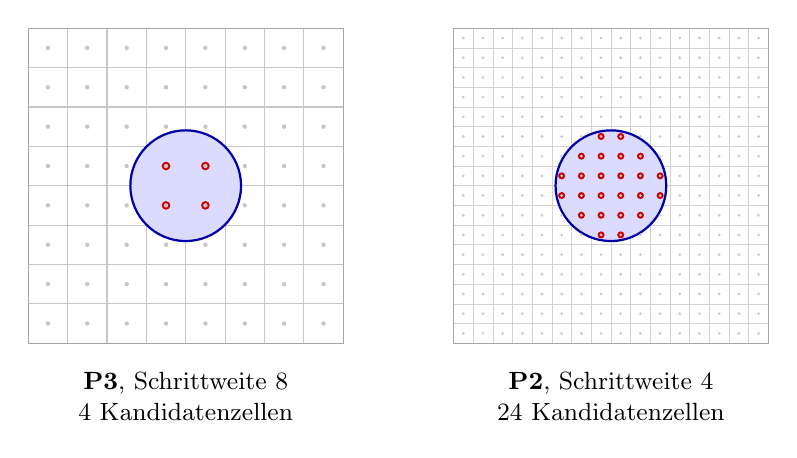
\begin{tikzpicture}[x=1cm,y=1cm]
  % ---------------- P3: Zellen 8 px = 0.5 cm ------------------------------
  \begin{scope}
    \draw[step=0.5,gray!45,thin] (0,0) grid (4,4);
    \draw[gray!70] (0,0) rectangle (4,4);
    \fill[blue!14] (2,2) circle (0.703);
    \draw[blue!65!black,thick] (2,2) circle (0.703);
    \foreach \x in {1.75,2.25}{\foreach \y in {1.75,2.25}{
      \fill[red!80!black] (\x,\y) circle (0.055);}}
    \foreach \x in {0.25,0.75,...,3.8}{\foreach \y in {0.25,0.75,...,3.8}{
      \fill[gray!45] (\x,\y) circle (0.028);}}
    \node[below,align=center,font=\small] at (2,-0.25)
         {\textbf{P3}, Schrittweite 8\\4 Kandidatenzellen};
  \end{scope}
  % ---------------- P2: Zellen 4 px = 0.25 cm -----------------------------
  \begin{scope}[shift={(5.4,0)}]
    \draw[step=0.25,gray!35,very thin] (0,0) grid (4,4);
    \draw[gray!70] (0,0) rectangle (4,4);
    \fill[blue!14] (2,2) circle (0.703);
    \draw[blue!65!black,thick] (2,2) circle (0.703);
    \foreach \x in {1.625,1.875,2.125,2.375}{
      \foreach \y in {1.625,1.875,2.125,2.375}{
        \fill[red!80!black] (\x,\y) circle (0.045);}}
    \foreach \p in {{1.375,1.875},{1.375,2.125},{2.625,1.875},{2.625,2.125},
                    {1.875,1.375},{2.125,1.375},{1.875,2.625},{2.125,2.625}}{
      \fill[red!80!black] (\p) circle (0.045);}
    \foreach \x in {0.125,0.375,...,3.9}{\foreach \y in {0.125,0.375,...,3.9}{
      \fill[gray!40] (\x,\y) circle (0.02);}}
    \node[below,align=center,font=\small] at (2,-0.25)
         {\textbf{P2}, Schrittweite 4\\24 Kandidatenzellen};
  \end{scope}
\end{tikzpicture}
\caption[Kandidatenzellen auf P3 und P2]{Warum ein feineres Gitter hilft.
Dargestellt ist ein Bildbereich von $64\times64$ Pixeln mit einem Objekt von
22,5\px{} Durchmesser -- dem Median des synthetischen Datensatzes. Punkte sind
Gitterzellenzentren, rot markiert sind jene, die in das Objekt fallen und damit
als positive Labelzuweisung in Frage kommen. In der gezeichneten Lage sind es 4
gegen 24; über alle Lagen des Objektzentrums gemittelt 6,2 gegen 24,9
(Tabelle~\ref{tab:p2zellen}). Bei einem ankerfreien Kopf ist diese Zahl das
Trainingssignal, das je Objekt zur Verfügung steht.}
\label{abb:p2zellen}
\end{figure}

Zwei Ablesungen sind entscheidend. Erstens: Für die kleinsten real auftretenden
Objekte steht auf P3 im ungünstigsten Fall nur \emph{eine} Kandidatenzelle zur
Verfügung, auf P2 sind es vier. Ein Objekt, dessen Zuweisung an einer einzigen
Zelle hängt, ist gegenüber der Diskretisierung des Gitters maximal empfindlich --
genau das Problem, das die Small-Target-Aware Label Assignment von YOLO26 auf der
Verlustseite mildert. Zweitens ist der Vorteil \emph{größenabhängig}: Bei
27,4\px{} bietet schon P3 neun Zellen, die zusätzlichen 37 auf P2 ändern wenig.
Die Erwartung lautet also nicht \enquote{P2 hilft}, sondern \enquote{P2 hilft
dort, wo die Objekte klein sind} -- und diese Erwartung ist prüfbar.

\subsection{Ergebnis}

\begin{table}[htbp]
\centering
\caption[Ergebnis des P2-Vergleichs]{Ergebnis des P2-Vergleichs. Oben nativer
Maßstab, unten bei der je Modell nach \mAPall{} auf \code{val} gewählten
Auflösung (\code{yolo26s}: 1600, \code{yolo26s-p2}: 1920); \code{test} blieb an
der Auswahl unbeteiligt. Fett ist je Spalte der bessere Wert -- die beiden
Modelle werden von der Zielgröße \emph{Zählfehler} und von \mAPfifty{}
\textbf{gegenläufig} geordnet (Abschnitt~\ref{sec:p2zaehlung}).}
\label{tab:p2ergebnis}
\footnotesize
\resizebox{\textwidth}{!}{%
\begin{tabular}{@{}lrrrrrrrr@{}}
\toprule
\textbf{Modell} & \code{test} \textbf{Zählung} &
\code{test} \textbf{Zählfehler} & \code{val} \mAPfifty{} &
\code{test} \mAPfifty{} & \code{test} \mAPseven{} & \code{test} \mAPall{} &
\code{test} $F_1$ & \code{test} $P$ / $R$ \\
\midrule
\multicolumn{9}{@{}l}{\itshape nativer Maßstab}\\
\code{yolo26s}    & \textbf{83/86} & \textbf{3,5\,\%} & 0,931 & 0,905 & 0,333 & 0,427 & 0,888 & 0,904 / 0,872 \\
\code{yolo26s-p2} & 79/86 & 8,1\,\% & \textbf{0,936} & \textbf{0,941} &
\textbf{0,387} & \textbf{0,450} & \textbf{0,933} & \textbf{0,975} / \textbf{0,895} \\
\midrule
\multicolumn{9}{@{}l}{\itshape bei der auf \code{val} gewählten \code{imgsz}}\\
\code{yolo26s} (1600)    & \textbf{83/86} & \textbf{3,5\,\%} & 0,939 & 0,905 & -- & 0,427 & 0,888 & 0,904 / 0,872 \\
\code{yolo26s-p2} (1920) & 81/86 & 5,8\,\% & \textbf{0,940} & \textbf{0,947} & -- &
\textbf{0,449} & \textbf{0,934} & \textbf{0,963} / \textbf{0,907} \\
\bottomrule
\end{tabular}}
\end{table}

Die theoretische Erwartung bestätigt sich: Bei praktisch identischer
Parameterzahl erreicht \code{yolo26s-p2} auf dem unberührten Testbild
\mAPfifty{} = 0,941 statt 0,905 und \mAPseven{} = 0,387 statt 0,333. Der Gewinn
entsteht dabei \emph{nicht} über die Boxpräzision -- die mittlere Treffer-IoU
sinkt sogar leicht von 0,729 auf 0,728 --, sondern über die Trennung von Objekt
und Hintergrund: Die Precision am Betriebspunkt steigt von 0,904 auf 0,975 bei
ebenfalls höherem Rückruf (0,872 auf 0,895). Das ist mit der Rechnung konsistent:
Ein feineres Gitter senkt die Auflösungsgrenze, an der ein Objekt überhaupt
detektierbar ist; es macht die Boxregression bei 20\px-Objekten aber nicht
genauer. Ein zweiter Befund steckt im Trainingsverlauf: \code{yolo26s} erreichte
sein bestes Modell in Epoche~5 und verbesserte sich danach 20 Epochen nicht mehr,
\code{yolo26s-p2} verbesserte sich bis Epoche~22 -- dasselbe Muster wie im dritten
Befund der Okklusionsablation: Wo mehr nutzbares Trainingssignal je Objekt vorliegt,
sättigt das Modell später.

\subsection{Der Vorteil ist größenabhängig}
\label{sec:p2aufloesung}

Die interessantere Prüfung ist nicht der Vergleich bei einer Auflösung, sondern
das Verhalten über die Auflösung -- denn die Rechnung in
Tabelle~\ref{tab:p2zellen} sagt vorher, \emph{wo} der Vorteil liegen muss.
Abbildung~\ref{abb:p2sweep} trägt beide Sweeps gegeneinander auf.

\begin{figure}[htbp]
\centering
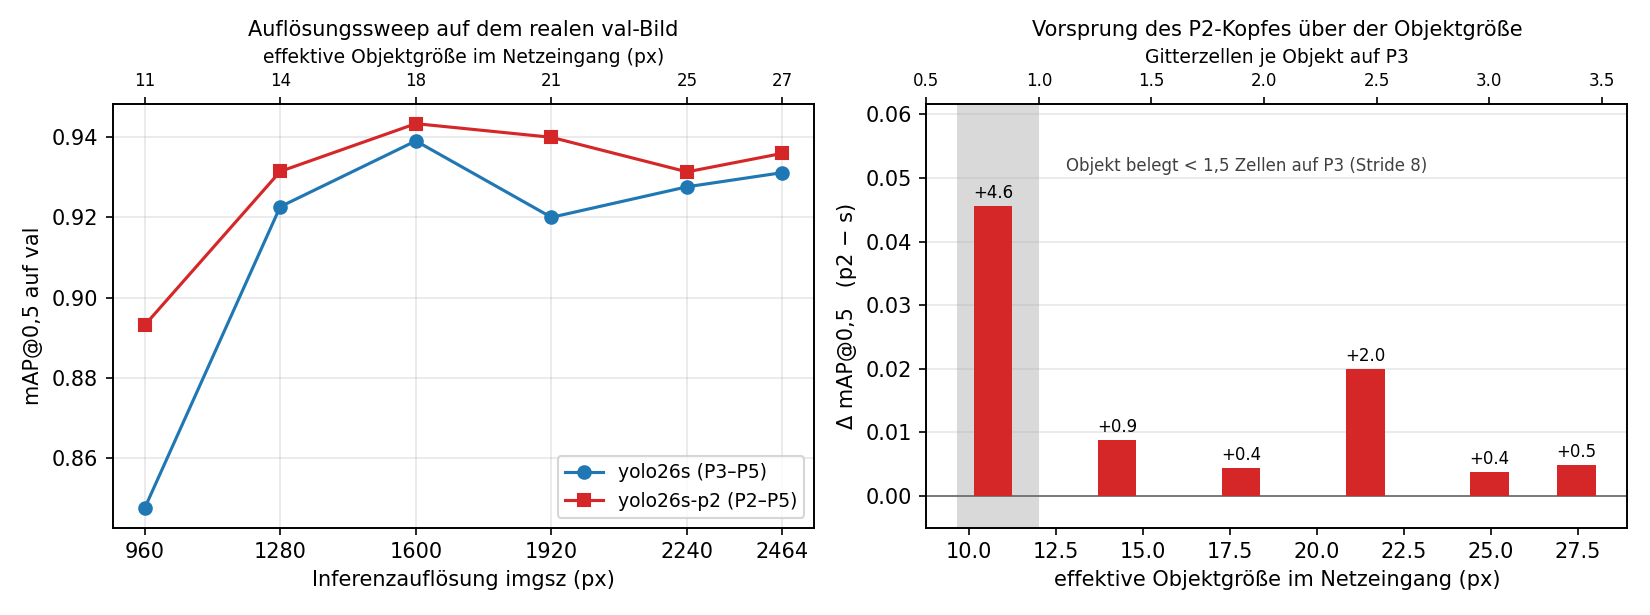
\includegraphics[width=\textwidth]{abbildungen/p2_sweep.png}
\caption[P2-Vorteil über der Auflösung]{Links: \mAPfifty{} auf dem realen
\code{val}-Bild über der Inferenzauflösung für beide Varianten; die obere Achse
nennt die zugehörige effektive Objektgröße im Netzeingang nach
Gleichung~\eqref{eq:deff}. Rechts: die Differenz beider Kurven. Der schattierte
Bereich markiert Objektgrößen unter $1{,}5$ Zellen auf P3, also den Bereich, in
dem die Rechnung aus Tabelle~\ref{tab:p2zellen} den größten Vorteil vorhersagt.}
\label{abb:p2sweep}
\end{figure}

Der Befund entspricht der Vorhersage: Bei \code{imgsz}=960 -- die Objekte
erreichen das Netz dann mit 10,7\px, also 1,3 Zellen auf P3 -- beträgt der
Vorsprung \textbf{4,6\PP}. Er ist damit rund zehnmal so groß wie bei den
Auflösungen, bei denen die Objekte über zwei Zellen belegen (0,4--0,9\PP{} bei
1600 und 1280). Anders formuliert: Der P2-Kopf leistet dasselbe wie eine
Verdopplung der Inferenzauflösung, solange die Objekte klein sind -- und wird
überflüssig, sobald sie groß genug sind. Das ist praktisch verwertbar: Wer die
Aufnahmeauflösung nicht frei wählen kann oder aus Laufzeitgründen bei kleiner
\code{imgsz} inferieren muss, gewinnt durch den P2-Kopf deutlich; wer ohnehin
hochskaliert, kaum. Der Punkt bei \code{imgsz}=1920 fällt mit $+2{,}0$\PP{} aus
diesem Muster; er verletzt die Monotonie und ist -- wie alle Differenzen dieser
Abbildung außer der bei 960 -- vom Konfidenzintervall
(Abschnitt~\ref{sec:bootstrap}) nicht zu unterscheiden.

\subsection{\mAPfifty{} und Zählfehler ordnen die Modelle gegenläufig}
\label{sec:p2zaehlung}

Der Vorteil des feineren Kopfes setzt sich \emph{nicht} in die Zielgröße der
Anwendung um. Am $F_1$-optimalen Betriebspunkt zählt \code{yolo26s-p2} auf
\code{test} 79 statt 86 Objekte -- ein Zählfehler von 8,1\,\% gegenüber 3,5\,\%
bei \code{yolo26s}, das dieselbe Aufnahme mit dem \emph{schlechteren}
\mAPfifty{} auswertet (0,905 gegen 0,941). Die Rangfolge kippt also, je nachdem
welche Größe man ansetzt.

Die Ursache ist die Schwellenwahl, nicht die Architektur: Das $F_1$-Optimum von
\code{yolo26s-p2} liegt bei $c^* = 0{,}379$ gegenüber $0{,}134$ und tauscht damit
Rückruf gegen Precision. Formal ist der Grund, dass $F_1$ beide Fehlerarten
\emph{gleich} gewichtet, der Zählfehler sich aber aus ihrer \emph{Differenz}
ergibt: Falsch-Positive und Falsch-Negative kompensieren sich in der Zählung
teilweise, im $F_1$ nie. Die beiden Optima müssen deshalb nicht zusammenfallen,
und hier tun sie es nicht.

Daraus folgt die praktisch wichtigste Aussage dieses Experiments: \textbf{Für
eine Zählanwendung ist mAP das falsche Auswahlkriterium, und der Betriebspunkt
wirkt stärker als die Architektur.} Der Betriebspunkt wäre direkt auf den
Zählfehler zu optimieren -- das wurde hier bewusst nicht getan, weil eine auf
\code{val} kalibrierte Zählschwelle die Aussagekraft der \code{test}-Zahlen
geschwächt hätte. Zu beachten ist der Umfang: Der Unterschied beruht auf
\emph{einem} Testbild mit 86 Objekten an je einem Betriebspunkt. Belastbar ist
der große Abstand von vier Objekten mit identifizierter Ursache, nicht eine
Rangfolge auf ein Objekt Genauigkeit.

\subsection{Einschränkungen und Konsequenz}

Drei Vorbehalte sind zu nennen. Erstens beruht der Vergleich auf \emph{je einem}
Trainingslauf pro Variante; die Streuung über Seeds ist unbekannt. Zweitens
liegen alle Differenzen außer der bei \code{imgsz}=960 innerhalb des
Bootstrap-Intervalls. Drittens ist der Vorteil bei \mAPall{} \emph{nicht}
konsistent: Über den Sweep hinweg ist \code{yolo26s-p2} bei drei von sechs
Auflösungen schlechter, was zur unveränderten Treffer-IoU passt -- P2 verbessert
das Finden, nicht das Lokalisieren.

Die Konsequenz für die Arbeit: Der P2-Kopf ist die wirksamste
\emph{architektonische} Maßnahme gegen das in
Abschnitt~\ref{sec:ioukleinobjekt} beschriebene Auflösungsproblem, und er ist
gegenüber der Alternative -- höhere Inferenzauflösung -- die
speichergünstigere Lösung, solange man die Trainingskosten einmalig aufbringen
kann. Für einen produktiven Einsatz wäre \code{yolo26s-p2} zu wählen; die in
dieser Arbeit dokumentierten Experimente~1 und~2 wurden auf der yolo11s-Baseline
gerechnet und bleiben davon unberührt, weil alle drei Modelle auf P3/P4/P5
dieselben Schrittweiten haben.

\section{Statistische Belastbarkeit und Fehleranalyse}
\label{sec:bootstrap}

Da je Split nur \emph{ein} Bild vorliegt, ist ein gewöhnlicher Bootstrap über
Bilder nicht möglich. Verwendet wird ein räumlicher Block-Bootstrap: Das Bild wird
in Kacheln zerlegt, über die mit Zurücklegen neu gezogen wird (400
Wiederholungen); die Blockbildung ist nötig, weil benachbarte Objekte nicht
unabhängig sind -- sie teilen Beleuchtung, Schärfe und Verdeckungssituation
\parencite{kuensch1989,efron1993}. Für \mAPfifty{} ergibt sich \code{val}
$0{,}892 \pm 0{,}051$ mit 95\,\%-Intervall $[0{,}766;\,0{,}965]$ (23 Kacheln) und
\code{test} $0{,}911 \pm 0{,}036$ mit $[0{,}844;\,0{,}974]$ (25 Kacheln). Alle in
diesem Kapitel berichteten Unterschiede unterhalb dieser Größenordnung sind als
Hinweis und nicht als Nachweis zu lesen; nicht betroffen ist der
Auflösungseffekt, dessen Größe von 47\PP{} das Intervall um ein Vielfaches
übersteigt.

\absatz{Falsch-Negative.} Sie treten fast ausschließlich bei sehr kleinen
Objekten am linken Bildrand von \code{test} (12--15\px), bei stark verdeckten
Enden tief im Stapel -- also dort, wo die Pipeline auch selbst kein Label mehr
vergäbe -- und bei Enden ohne sichtbaren hellen Kranz auf. Letzteres ist der
Fehlertyp, der auf die verbleibende Domänenlücke zurückgeht: Alle vier Clean
Plates sind bei diffusem Licht aufgenommen.

\absatz{Falsch-Positive.} Ihre Ursache unterscheidet sich zwischen den beiden
Bildern, und die Unterscheidung ist nicht kosmetisch. Auf \code{val} haben 9 der
11 Falsch-Positiven \emph{keinerlei} Überlappung mit einer Ground-Truth-Box; ein
Teil von ihnen sitzt auf erkennbaren Rohröffnungen, die in der Annotation fehlen.
Bei 88 handannotierten Objekten schlägt jede fehlende Annotation mit etwa
1,1\PP{} Precision zu Buche, die berichteten Precision-Werte sind also eine
\textbf{Untergrenze}. Die übrigen entstehen an dunklen Löchern im Maschendraht
und an Schattenspalten zwischen Rohren -- genau die Strukturen, gegen die die
Negativbilder gerichtet sind; dass sie dort noch auftreten, spricht dafür, dass
deren Anteil von 9,7\,\% eher an der Untergrenze des Sinnvollen liegt. Auf
\code{test} liegt der Fall völlig anders, und er ist Gegenstand des folgenden
Abschnitts.

\section{Ein systematischer Größenversatz der Boxen}
\label{sec:boxversatz}

Im Qualitativbild des Testbildes (Abbildung~\ref{abb:qualitativ} im Anhang)
liegen an mehreren Stellen eine rote und eine blaue Box nahezu deckungsgleich --
dieselbe Stirnfläche wird also gleichzeitig als Falsch-Positiv \emph{und} als
Falsch-Negativ gezählt. Das ist kein Darstellungsfehler, sondern die unmittelbare
Folge der Zuordnungsregel: Eine Detektion gilt nur als Treffer, wenn ihre IoU mit
der Ground-Truth-Box mindestens 0,5 beträgt. Liegt sie darunter, bleibt die
Detektion unzugeordnet (rot) und die Ground-Truth-Box unbedient (blau) -- ein und
dasselbe Objekt erzeugt zwei Fehler.

Auf \code{test} betrifft das \textbf{sechs der acht Falsch-Positiven}. Ihre IoU
liegt zwischen 0,401 und 0,497, in zwei Fällen wird die Schwelle um weniger als
0,005 verfehlt; alle sechs sitzen mit Konfidenzen zwischen 0,52 und 0,84 auf
annotierten Objekten. Senkt man allein die Zuordnungsschwelle von 0,50 auf 0,40,
so ergeben sich 81 Treffer, 2 Falsch-Positive und 5 Falsch-Negative statt
75/8/11 -- Abbildung~\ref{abb:qualitativ} im Anhang zeigt beide Fassungen
desselben Bildes mit identischer Detektionsmenge. Auf \code{val} tritt der
Effekt nicht auf; dort ändert dieselbe Absenkung nichts.

Die naheliegende Frage, ob damit nicht schon alles behoben sei, ist zu
verneinen. Eine niedrigere Schwelle verschiebt die \emph{Messkonvention}, nicht
die Ursache: Sie erklärt sechs Fehler weg, ohne dass die Boxen genauer würden,
und 0,50 ist der Bezugswert von PASCAL VOC und COCO
\parencite{everingham2010,lin2014coco}. Ein berichteter Wert bei 0,40 wäre nicht
mehr mit Literaturzahlen vergleichbar und stünde im Verdacht, die Metrik dem
Ergebnis angepasst zu haben. Die abgesenkte Schwelle ist deshalb ein
\emph{Diagnosewerkzeug} -- sie trennt Zuordnungsartefakte von echten Fehlern --,
und die Korrektur gehört an die Labelkonvention.

\absatz{Die Boxen sind systematisch zu klein.} Die Ursache lässt sich messen.
Tabelle~\ref{tab:boxversatz} vergleicht für jede Detektion, die eindeutig auf
einem annotierten Objekt sitzt ($\mathrm{IoU} > 0{,}3$), die vorhergesagte mit
der annotierten Boxgröße.

\begin{table}[htbp]
\centering
\caption[Größenversatz der Boxen]{Vergleich der vorhergesagten mit der
annotierten Boxgröße. Als Boxgröße dient $\sqrt{\text{Fläche}}$, der
Zentrumsversatz ist in Objektdurchmessern angegeben. \code{sval} ist der
synthetische Split, dessen Labels der Generator selbst erzeugt hat.}
\label{tab:boxversatz}
\footnotesize
\begin{tabular}{@{}lrrrrr@{}}
\toprule
\textbf{Split} & \textbf{Paare} & \textbf{Objekt-\Oe{} (Median)} &
\textbf{pred/GT} & \textbf{GT $-$ pred} & \textbf{Zentrumsversatz} \\
\midrule
\code{test} (real)        &   82 & 22,3\px & 0,884 & $+2{,}53$\px & 0,049\,\Oe \\
\code{val} (real)         &   75 & 27,5\px & 0,961 & $+1{,}16$\px & 0,054\,\Oe \\
\code{sval} (synthetisch) & 1064 & 22,0\px & \textbf{1,012} & $-0{,}29$\px & -- \\
\bottomrule
\end{tabular}
\end{table}

Der Befund ist eindeutig. Auf dem synthetischen Split trifft das Modell die
Boxgröße auf 1\,\% genau; auf den realen Bildern liegt sie 4\,\% (\code{val})
bzw.\ 12\,\% (\code{test}) darunter. Der Versatz ist dabei in \emph{absoluten}
Pixeln annähernd konstant und trifft deshalb die kleinsten Objekte am härtesten:
Bei Objekten unter 18\px{} beträgt das Verhältnis nur noch 0,830, bei über
26\px{} dagegen 0,894. Der Zentrumsversatz liegt mit rund 0,05
Objektdurchmessern (etwa 1\px) dagegen im Bereich der Annotationsgenauigkeit --
es handelt sich also um einen Größen-, nicht um einen Positionsfehler.

\begin{figure}[htbp]
\centering
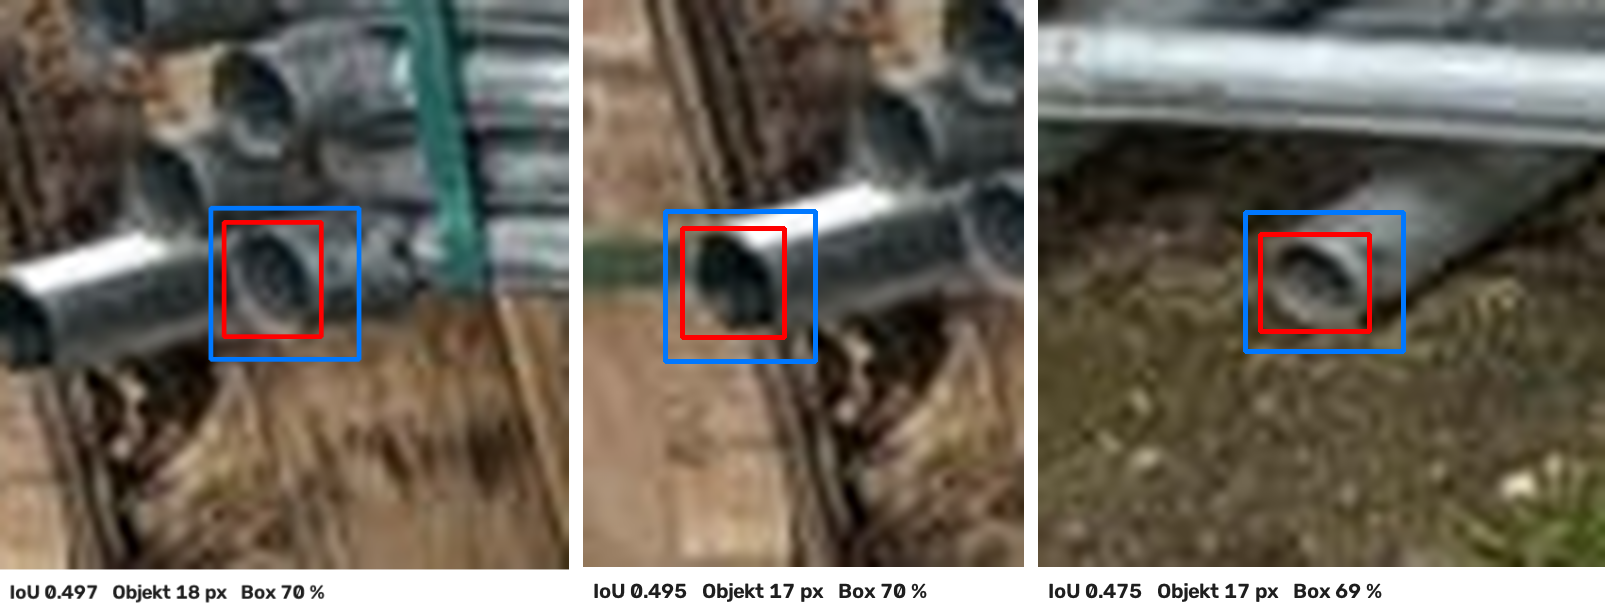
\includegraphics[width=\textwidth]{abbildungen/boxversatz.png}
\caption[Rote und blaue Box am selben Objekt]{Drei der sechs betroffenen Stellen
aus dem Testbild, neunfach vergrößert. Blau die Handannotation, rot die
Detektion. Alle drei Objekte sind gefunden, die vorhergesagte Box umfasst aber
nur etwa 70\,\% der annotierten Kantenlänge; die IoU bleibt damit knapp unter der
Zuordnungsschwelle 0,5, und dasselbe Objekt zählt als Falsch-Positiv \emph{und}
als Falsch-Negativ.}
\label{abb:boxversatz}
\end{figure}

\absatz{Modellfehler oder Labelkonvention?} Weil das Modell auf dem synthetischen
Split die Boxgröße nahezu exakt reproduziert, liegt die Ursache nicht in der
Boxregression, sondern in der \emph{Labelkonvention}: Die Generatorboxen folgen
der $\alpha > 0{,}5$-Kontur der Alphamaske
(Abschnitt~\ref{sec:sichtbarkeit}), die Handannotation umschließt das Objekt
großzügiger. Anforderung~A5 -- identische Labeldefinition in Quelle und Ziel --
ist damit nur \emph{annähernd} erfüllt; der Restversatz beträgt messbar 1,2 bis
2,5\px. Abbildung~\ref{abb:boxversatz} zeigt zugleich die Gegenprobe: Es sind die
kleinsten und kontrastärmsten Objekte, bei denen sich die Detektion auf die
dunkle Bohrung zusammenzieht, während die Annotation den hellen Kranz mit
einschließt. Ein Teil des Versatzes ist damit auch echte
Lokalisierungsschwierigkeit und nicht allein Konvention.

\absatz{Was der Versatz kostet.} Eine Sensitivitätsrechnung schätzt die
Größenordnung: Weitet man alle vorhergesagten Boxen um den gemessenen medianen
Fehlbetrag je Seite auf (1,27\px{} auf \code{test}, 0,58\px{} auf \code{val}) und
wertet neu aus, so ergibt sich Tabelle~\ref{tab:boxsens} im Anhang.

Auf \code{test} steigt \mAPseven{} von 0,320 auf 0,714 und \mAPall{} von 0,437
auf 0,604; auf \code{val}, wo der Versatz weniger als halb so groß ist, bewegt
sich entsprechend wenig. Damit ist auch der in
Abschnitt~\ref{sec:hauptergebnis} auffällige Unterschied zwischen den Splits
erklärt: Er geht nur zu einem Teil auf die kleinere Objektgröße in \code{test}
zurück, überwiegend aber auf die dort um 1,4\px{} großzügigere Annotation. Die
berichteten Werte für \mAPseven{} und \mAPall{} auf \code{test} sind folglich
\textbf{pessimistisch} -- sie messen zu einem erheblichen Teil eine
Konventionsdifferenz und nicht die Lokalisierungsgüte des Modells. Für
\mAPfifty{}, das $F_1$ und den Zählfehler -- die für die Anwendung maßgeblichen
Größen -- bleibt der Effekt klein.

\absatz{Konsequenz.} Die Korrektur ist einfach und sollte vor jeder weiteren
Optimierung erfolgen: Die Boxen des Generators sind an die Annotationskonvention
anzupassen, indem die Boxschwelle von $\alpha > 0{,}5$ herabgesetzt oder die
fertige Box um etwa 1\px{} je Seite aufgeweitet wird. Sauberer, aber teurer wäre
der umgekehrte Weg -- die 174 Handlabels nach derselben Regel neu zu ziehen, nach
der der Generator seine Boxen bildet. Solange beides nicht geschehen ist, sind
die Lokalisierungsmetriken dieser Arbeit untereinander vergleichbar, nicht aber
gegen Literaturwerte.
